% !TeX root = RJwrapper.tex
\title{NMAforest: An R Package for Generating Forest Plots in Network Meta-Analysis with Decomposition of Direct, Indirect, and Study-Level Evidence Contributions}

\author{by Yanqi Zhang, Chong Wang, Annette O'Connor}

\maketitle

\abstract{
We present \CRANpkg{NMAforest}, an R package designed to visualize results from network meta-analysis (NMA) by producing forest plots that explicitly decompose and visualize the contributions of direct and indirect evidence to treatment effect sizes. While existing packages provide tools to summarize treatment effect estimates and confidence intervals in NMA, they typically do not attribute how much each study, comparison, or path contributes to these results. \CRANpkg{NMAforest} addresses this limitation by integrating effect estimation summaries with the treatment network’s structural information and the Hat matrix, enabling a transparent decomposition of evidence flows. The package computes effect estimates for direct comparisons, indirect routes through specific network paths, and the overall NMA estimate, accompanied by 95\% confidence intervals. The forest plot enables visualization of the relative contribution of each evidence component using proportion bars aligned with the estimates, facilitating a clearer interpretation of the strength and source of evidence.
}

\section{Introduction}
Network meta-analysis (NMA)  extends pairwise meta-analysis by allowing simultaneous comparisons among multiple treatments, even in the absence of head-to-head comparisons. This framework has become essential in comparative effectiveness research across disciplines such as clinical medicine, epidemiology, and public health, where evidence networks are often sparse or partially connected.

While NMA enables indirect estimations and an approach to combining direct and indirect evidence, it also introduces substantial complexity in interpreting how treatment effect estimates are derived. Specifically, each estimate typically combines direct evidence from studies that directly compared the treatments and indirect evidence accumulated via intermediate comparisons across the network. Understanding this composition is crucial for evaluating the robustness of conclusions, detecting influential studies or comparisons, and assessing the consistency between direct and indirect evidence.

One approach to quantifying evidence contribution is the projection matrix (commonly referred to as the Hat matrix), which arises from the linear model formulation of NMA introduced by \citet{Lu2011}. This approach formalizes the combination of evidence and enables estimation of both treatment effects and their associated uncertainty. Building upon this, \citet{Konig2013} demonstrated how the Hat matrix can be interpreted in terms of evidence flow, assigning proportions of each treatment effect estimate to different direct comparisons. More recently, \citet{Papakonstantinou2018} extended this interpretation by introducing the concept of evidence streams: directed paths through the treatment network that quantify how evidence propagates indirectly between treatments. Their algorithms use flow decomposition to allocate contributions from direct comparisons across all paths in a way that is consistent with the underlying model assumptions.

Despite this theoretical progress, practical tools for decomposing and visualizing evidence contributions remain limited. For example, the popular \CRANpkg{netmeta} R package \citep{netmeta-jss} implements frequentist NMA and computes Hat matrices but does not provide built-in methods to enumerate evidence paths or produce contribution-aware forest plots. General-purpose visualization tools, such as the R package \CRANpkg{forestplot} \citep{forestplot-pkg}, are designed only for plotting and do not perform statistical calculations or differentiate between sources or relative contributions of evidence. This lack of transparency can limit interpretability and hinder effective communication of NMA results to stakeholders.

To address these challenges, we introduce the \CRANpkg{NMAforest} package, which integrates statistical estimates, evidence flow decomposition, and contribution visualization in a unified workflow. By combining network structure and Hat matrix-based proportions with standard forest plot representations, \CRANpkg{NMAforest} enables researchers to generate richly annotated plots that clearly delineate the origins of each estimate and the influence of each study and path within the network. The \CRANpkg{NMAforest} package is available from CRAN at \url{https://CRAN.R-project.org/package=NMAforest}.

\section{Motivation}
The motivation for developing \CRANpkg{NMAforest} stems from the practical challenges faced by researchers and decision-makers who need to interpret and communicate NMA results. Pairwise meta-analysis and corresponding forest plots are effective for presenting treatment effect estimates and their uncertainty. Pairwise meta-analysis and forest plots also provide the weight that individual studies provide to treatment effect estimates. However, NMA is limited in the detail it conveys about where the evidence comes from. In practice, this often leads to questions such as: How much of the estimated effect relies on direct comparisons? Which indirect paths contribute the most information? Could the result be dominated by a small subset of studies?

These questions are particularly important in applications where evidence transparency and reproducibility are critical. For example, health technology assessments, guideline development, and policy decisions often require a clear audit trail showing how each piece of evidence informs the final estimate. While the Hat matrix and evidence stream decomposition methods provide a rigorous statistical basis for such attribution, extracting and interpreting these contributions typically requires multiple manual steps and specialized code.

\CRANpkg{NMAforest} was designed to fill this gap by offering an integrated set of tools that connect statistical estimation with intuitive visualization. The package builds directly upon the outputs of \CRANpkg{netmeta}, leveraging its estimates and Hat matrix computations to break down treatment comparisons into three main components: direct estimates derived from head-to-head studies, indirect estimates based on evidence propagating through specific paths in the network, and the overall NMA estimate that combines all available evidence.

Beyond estimating and displaying these components, \CRANpkg{NMAforest} provides a structured approach to display them graphically. In each forest plot, the effect size estimates for the direct, indirect, and NMA components are aligned with horizontal bars that represent the relative contribution of each evidence path. This combination of quantitative and visual decomposition improves transparency, facilitates critical appraisal, and supports sensitivity analyses by making the influence of each evidence path explicit.

In this way, the package aims to make advanced evidence attribution methods accessible to a broader audience and to support a more informed interpretation of complex NMA results.

\section{Functionality}

The main function provided by the package is:

\begin{itemize}
  \item \texttt{NMAforest()}: Creates a forest plot that decomposes evidence contributions for a specified treatment comparison. The function also returns a structured statistical output containing study labels, treatment effect estimates for direct, indirect, and NMA comparisons, together with their standard errors, confidence intervals, and relative weights. Importantly, the output also includes proportion values that attribute contributions across overall estimates, paths, and individual studies.
\end{itemize}

This function supports the following arguments:

\begin{description}

 \item[\texttt{data}] - A data frame in long format containing the input data. Required columns include \texttt{study} (study label), \texttt{t} (treatment), and appropriate outcome data:
    \begin{itemize}
      \item For binary outcomes: \texttt{r} (events) and \texttt{N} (sample size)
      \item For continuous outcomes: \texttt{y} (mean), \texttt{sd} (standard deviation), and \texttt{N} (sample size)
    \end{itemize}

  \item[\texttt{sm}] - Summary measure for the treatment effect. Supported values include \texttt{"OR"} (odds ratio), \texttt{"RR"} (risk ratio), \texttt{"MD"} (mean difference), and \texttt{"SMD"} (standardized mean difference), etc.

  \item[\texttt{reference}] - The reference treatment against which others are compared.

  \item[\texttt{model}] - Type of NMA model to use. The options are \texttt{"random"} or \texttt{"fixed"}.

  \item[\texttt{comparison}] - A character vector of length two, indicating the pair of treatments to be compared.

  \item[\texttt{study}] - Column name identifying the study label.

  \item[\texttt{treat}] - Column name for treatment assignment.

  \item[\texttt{event}] - Column name for event counts (used for binary outcomes).

  \item[\texttt{N}] - Column name for total sample size (used for binary outcomes and continuous outcomes).

  \item[\texttt{mean}] - Column name for mean values (used for continuous outcomes).

  \item[\texttt{sd}] - Column name for standard deviations (used for continuous outcomes).

  \item[\texttt{study\_id}] - Column name used to uniquely identify each study arm (default = "\texttt{study\_id}"). If the column is not present in the original dataset, the updated data frame will be returned with this column added. 

  \item[\texttt{study\_path}] - Logical argument. If \texttt{TRUE}, the function decomposes indirect path contributions further into study-level components. If \texttt{FALSE}, only the overall indirect effect and its individual paths are shown, without breaking them down to individual study combinations. For large or highly connected networks, setting \texttt{study\_path} = \texttt{FALSE} is recommended to suppress study-level path decomposition and generate a cleaner, more interpretable summary plot.

\end{description}

\section{Method}

The \CRANpkg{NMAforest} package implements a structured approach to quantify and visualize the evidence contributing to network meta-analysis (NMA) estimates. It decomposes each comparison into direct and indirect evidence, identifies study-level contributions, and displays these as aligned effect estimates and proportion bars. The following subsections describe the computations used to generate each component of the plot.

All computations implemented in the \CRANpkg{NMAforest} package are based on the standard frequentist network meta-analysis model as implemented in \CRANpkg{netmeta}. Consequently, the proposed decomposition and visualization of evidence rely on the assumptions of \textbf{transitivity} and \textbf{consistency} \citep{Ahn2021NMA}. Transitivity assumes that studies comparing different treatment pairs are sufficiently comparable with respect to effect-modifying factors, while consistency assumes agreement between direct and indirect evidence for the same treatment contrast. 

\subsection{Overall Direct Effect and Study-Level Contributions}

The overall direct effect for a given treatment comparison (e.g., \texttt{x} vs. \texttt{y}) is estimated using the \texttt{netmeta()} function. This produces an effect estimate $\hat{\theta}^{\mathrm{D}}_{xy}$ with an associated standard error and a 95\% confidence interval. The superscript notation is used to distinguish direct effect estimates from indirect ($\hat{\theta}^{\mathrm{I}}_{xy}$) estimates considered elsewhere.

To determine how much each study contributes to the direct estimate, we use the \textbf{hat matrix} $H$, derived from the linear projection of NMA comparisons onto the space of observed direct effects:

\[
H = Y (X^\top (V^D)^{-1} X)^{-1} X^\top (V^D)^{-1}
\]

where:
\begin{itemize}
  \item $X$ is a $D \times (T - 1)$ matrix describing observed direct comparisons, where:
  \begin{itemize}
    \item $D$ is the number of treatment comparisons informed by direct evidence,
    \item $T$ is the total number of treatments in the network.
  \end{itemize}
  \item $Y$ is a $\binom{T}{2} \times (T - 1)$ matrix for all treatment contrasts,
  \item $V^D$ is a $D \times D$ covariance matrix of direct estimates.
\end{itemize}

The total contribution (flow) of the $xy$ direct comparison to the overall NMA estimate is captured by the corresponding diagonal entry of the hat matrix, denoted as $\left| H^{xy}_{xy} \right|$ \citep{Papakonstantinou2018}.

In a \textbf{random-effects model}, between-study variability is captured using the heterogeneity parameter $\tau^2$ (tau-squared). This represents the variance of true treatment effects across studies. 

Each study $i$ contributing to the $xy$ direct comparison receives a weight:

\[
w^{xy}_{i} = \frac{1}{\left( \mathrm{SE}_i^{xy} \right)^2
 + \tau^2}
\]

The proportional contribution of study $i$ to the overall direct estimate for the comparison $x$ vs.\ $y$ is then \citep{Riley2018}:

\[
\text{Proportion}_i^{xy} = 
\frac{w_i^{xy}}{\sum\limits_{i' \in S_{xy}} w_{i'}^{xy}} 
\cdot \left| H^{xy}_{xy} \right|
\]

where:
\begin{itemize}
  \item $S_{xy}$ is the set of studies with direct data on the $xy$ comparison,
  \item $\text{Proportion}_i^{xy}$ is the contribution of study $i$ to the NMA estimate via the $xy$ direct comparison.
\end{itemize}

\subsection{Indirect Paths and Study-Combination Contributions}

Indirect evidence for comparison $x$ vs.\ $y$ arises via intermediate treatments. All indirect paths (e.g., $x \rightarrow v \rightarrow y$) are identified using \texttt{igraph::all\_simple\_paths()} \citep{igraph2006, igraph2025}. Each path is treated as a sequence of direct comparisons, and the indirect estimate for one certain path is calculated as:

\[
\hat{\theta}^{\mathrm{I}}_{xy} = \hat{\theta}^{\mathrm{D}}_{xv} + \hat{\theta}^{\mathrm{D}}_{vy}
\]

The variance of this estimate accounts for the variances of the contributing comparisons and their covariance. If any two comparisons along the path originate from the same study, the covariance between them is approximated using a constant correlation approach:

\[
\mathrm{Cov}(\hat{\theta}^{\mathrm{D}}_{xv}, \hat{\theta}^{\mathrm{D}}_{vy}) = \rho \cdot \mathrm{SE}^{xv}_i \cdot \mathrm{SE}^{vy}_j
\] where $\rho = 0.5$ by default. If no study includes both comparisons, the covariance term is set to zero. 

In multi-arm trials, treatment comparisons within the same study are statistically correlated and require specification of within-study correlations to construct the variance--covariance matrix. Following standard practice in \CRANpkg{netmeta}, we adopt a constant-correlation assumption with $\rho = 0.5$ \citep{LuAdes2006}. This assumption affects the estimated variances and covariances of treatment effects and therefore influences the width of confidence intervals, while leaving point estimates unchanged.

The total variance of the indirect estimate is then:

\[
\mathrm{Var}(\hat{\theta}^{\mathrm{I}}_{xy}) = \mathrm{Var}(\hat{\theta}^{\mathrm{D}}_{xv}) + \mathrm{Var}(\hat{\theta}^{\mathrm{D}}_{vy}) + 2 \cdot \mathrm{Cov}(\hat{\theta}^{\mathrm{D}}_{xv}, \hat{\theta}^{\mathrm{D}}_{vy})
\]

Each indirect path is assigned a \textbf{flow value} $\mathrm{Flow}^{xy}_k$, which quantifies the contribution of that specific indirect path to the overall NMA estimate. These flow values are computed using an adapted \texttt{comparisonStreams()} function originally developed by \citet{Papakonstantinou2018}. These flow values satisfy the constraint:

\[
\sum_{\text{indirect paths } k} \mathrm{Flow}^{xy}_k = 1 - \left| H^{xy}_{xy} \right|
\]

Within each path, we identify contributing study combination $(i, j)$, where:
\begin{itemize}
  \item $i$ is a study contributing to comparison $xv$,
  \item $j$ is a study contributing to comparison $vy$.
\end{itemize}

The weights for these studies are defined as:

\[
w_i^{xv} = \frac{1}{\left( \mathrm{SE}_i^{xv} \right)^2 + \tau^2}, \quad
w_j^{vy} = \frac{1}{\left( \mathrm{SE}_j^{vy} \right)^2 + \tau^2}
\]

Then, the proportional contribution of study combination $(i, j)$ to the indirect path is:

\[
\text{Proportion}_{(i,j)}^{xy} =
\left( \frac{w_i^{xv}}{\sum_{i' \in S_{xv}} w_{i'}^{xv}} \right)
\cdot
\left( \frac{w_j^{vy}}{\sum_{j' \in S_{vy}} w_{j'}^{vy}} \right)
\cdot \mathrm{Flow}^{xy}_k
\]
where:
\begin{itemize}
  \item $S_{xv}$ is the set of studies with direct data on the $xv$ comparison,
  \item $S_{vy}$ is the set of studies with direct data on the $vy$ comparison,
  \item $\text{Proportion}_{(i,j)}^{xy}$ is the contribution of study combination $(i, j)$ to the NMA estimate via the $xy$ direct comparison.
\end{itemize}

These combination-level contributions appear as individual rows under each path in the expanded forest plot, along with their corresponding effect estimates and proportion bars.

\subsection{Evidence Flow Algorithm}
This subsection briefly describes how indirect evidence is represented and partitioned across paths using the adapted \texttt{comparisonStreams()} procedure implemented in \CRANpkg{NMAforest}. For a target comparison (e.g., $x$ vs.\ $y$), the procedure starts from the hat matrix obtained from the \CRANpkg{netmeta} model, which quantifies the contribution of each observed direct comparison to the network estimate.

Indirect evidence is represented through paths that connect $x$ to $y$ via one or more intermediate treatments. Each indirect path is defined as an ordered sequence of direct comparisons (for example, $x \rightarrow v \rightarrow y$). The absolute values of the corresponding hat-matrix entries are treated as available contribution along each direct comparison involved in the path.

The algorithm iteratively identifies admissible indirect paths from $x$ to $y$ and assigns each path a contribution determined by the smallest remaining contribution among the direct comparisons forming that path. Once a path-level contribution is assigned, it is removed from the available contribution of all comparisons along the path. This ensures that indirect evidence is allocated across paths without double counting.

The final output is a collection of indirect paths, each associated with a nonnegative contribution weight. These path-level contributions are used by \CRANpkg{NMAforest} to display indirect evidence in the forest plot, allowing indirect information to be interpreted in terms of specific treatment sequences.

\subsection{Overall NMA Effect and Evidence Attribution}

The overall NMA effect $\hat{\theta}^{\mathrm{NMA}}_{xy}$ and its confidence interval are computed using \texttt{netmeta()}, combining all direct and indirect evidence for comparison $x$ vs.\ $y$.

The contribution bar displayed in the NMA effect row represents a full decomposition of all sources of evidence. It is constructed by summing the proportion contributed by the direct comparison and the proportions from all indirect paths, which ensures that 100\% of the evidence contributing to the NMA estimate is accounted for. As a result, users can interpret the overall estimate in terms of clearly attributed contributions from specific direct studies and indirect study combinations, facilitating transparent and interpretable visualizations.

\section{Usage}

\subsection{Required data format}

The \texttt{NMAforest()} function expects the input data to be in long format, with
one row per study arm. The following columns are required, either using the default
names listed below or specified explicitly via function arguments:

\begin{itemize}
  \item \texttt{treat}: treatment label for each arm;
  \item \texttt{study}: study identifier or label;
  \item \texttt{n}: sample size for each arm;
  \item \texttt{event}: number of events per arm (for binary outcomes);
  \item \texttt{mean}, \texttt{sd}: mean and standard deviation (for continuous outcomes).
\end{itemize}

An optional column \texttt{study\_id} may be provided to uniquely identify studies.
If \texttt{study\_id} is not supplied, \texttt{NMAforest()} automatically generates
this column and returns the updated data frame as part of the output.

\subsection{Output Structure}
The \texttt{NMAforest()} function returns a structured list that includes both a contribution-annotated forest plot and numerical outputs summarizing treatment effects and evidence contributions. The first element of this list is a \texttt{ggplot2} object named \texttt{\$plot}, which visualizes the decomposition of evidence. The forest plot consists of two aligned panels:

\begin{itemize}
  \item \textbf{Effect Size Panel (Left)}: Displays point estimates and 95\% confidence intervals for:
    \begin{itemize}
      \item The overall direct effect;
      \item Individual study-level direct comparisons;
      \item The overall indirect effect;
      \item Each indirect path;
      \item Optional: study combinations within indirect paths;
      \item The overall NMA effect estimate.
      \item \textbf{Visual weighting}: The size of each point estimate is scaled in proportion to its corresponding \texttt{proportion} value, so that larger contributions appear as larger points.
    \end{itemize}

  \item \textbf{Proportion Panel (Right)}: Displays horizontal bars aligned with each effect size row, representing the relative contribution (proportion) of each evidence source:
    \begin{itemize}
      \item Direct proportions are computed using the Hat matrix (\texttt{H});
      \item Indirect proportions are derived from the \texttt{comparisonStreams()} function \citet{Papakonstantinou2018}, adapted from the \texttt{flow\_contribution} package;
      \item When \texttt{study\_path = TRUE}, the function further disaggregates flow across combinations of studies along each path.
    \end{itemize}
\end{itemize}

In addition to the plot, \texttt{NMAforest()} returns the following components as part of the output list:

\begin{itemize}
  \item \texttt{\$output}: A data frame containing study label names, treatment effect estimates for direct, indirect, and NMA comparisons, along with standard errors, confidence intervals, relative weights, and proportion values for overall estimates, paths, and studies;
  \item \texttt{\$updated\_df}: The input data frame with a unique \texttt{study\_id} column added (if not already present), used for internal processing and traceability.
\end{itemize}

These outputs allow users not only to visualize the structure and sources of evidence but also to extract, inspect, and reuse the underlying quantitative components in downstream analyses.

\subsection{Example Case}

\begin{verbatim}
# Example 1: Binary outcome data
data(example_data)

NMAforest(
  data = example_data,
  sm = "OR",
  reference = "x",
  model = "random",
  comparison = c("x", "y"),
  study = "study",
  treat = "t",
  event = "r",
  N = "n",
  study_id = "id",
  study_path = TRUE
)

# Example 2: Continuous outcome data
data("parkinson", package = "pcnetmeta")

NMAforest(
  data = parkinson,
  sm = "MD",
  reference = "1",
  model = "random",
  comparison = c("1", "3"),
  study = "s.id",
  treat = "t.id",
  mean = "mean",
  sd = "sd",
  N = "n",
  study_path = TRUE
)
\end{verbatim}

\subsection{Example Datasets}

To demonstrate that \CRANpkg{NMAforest} operates consistently across different outcome types, we present two example datasets in arm-level format: one with binary outcomes and one with continuous outcomes. In both cases, each row corresponds to a study arm and provides the quantities required by \CRANpkg{NMAforest} to perform network meta-analysis and visualize evidence decomposition.

The first example dataset contains binary outcome data from 13 clinical trials comparing four treatments: \texttt{x}, \texttt{y}, \texttt{u}, and \texttt{v}. Each row records the study label (\texttt{study}), treatment label (\texttt{t}), number of events (\texttt{r}), total sample size (\texttt{n}), and a study identifier (\texttt{id}). These variables correspond directly to the arguments \texttt{study}, \texttt{treat}, \texttt{event}, \texttt{N}, and \texttt{study\_id} used in \CRANpkg{NMAforest}.

The second example dataset uses the \texttt{parkinson} data from the \CRANpkg{pcnetmeta} package and contains continuous outcome summary statistics from 7 clinical trials comparing five treatments labeled \texttt{1}--\texttt{5}. Each row includes the study identifier (\texttt{s.id}), treatment identifier (\texttt{t.id}), arm-level sample mean (\texttt{mean}), standard deviation (\texttt{sd}), and sample size (\texttt{n}). These correspond to the arguments \texttt{study}, \texttt{treat}, \texttt{mean}, \texttt{sd}, and \texttt{N} required for continuous outcomes. 

In both examples, the treatment networks are connected and include multi-arm studies, allowing the target comparisons to be informed by both direct and indirect evidence. 

\subsection{Binary Data Example Plot and Output}

\begin{figure}[htbp]
  \centering
  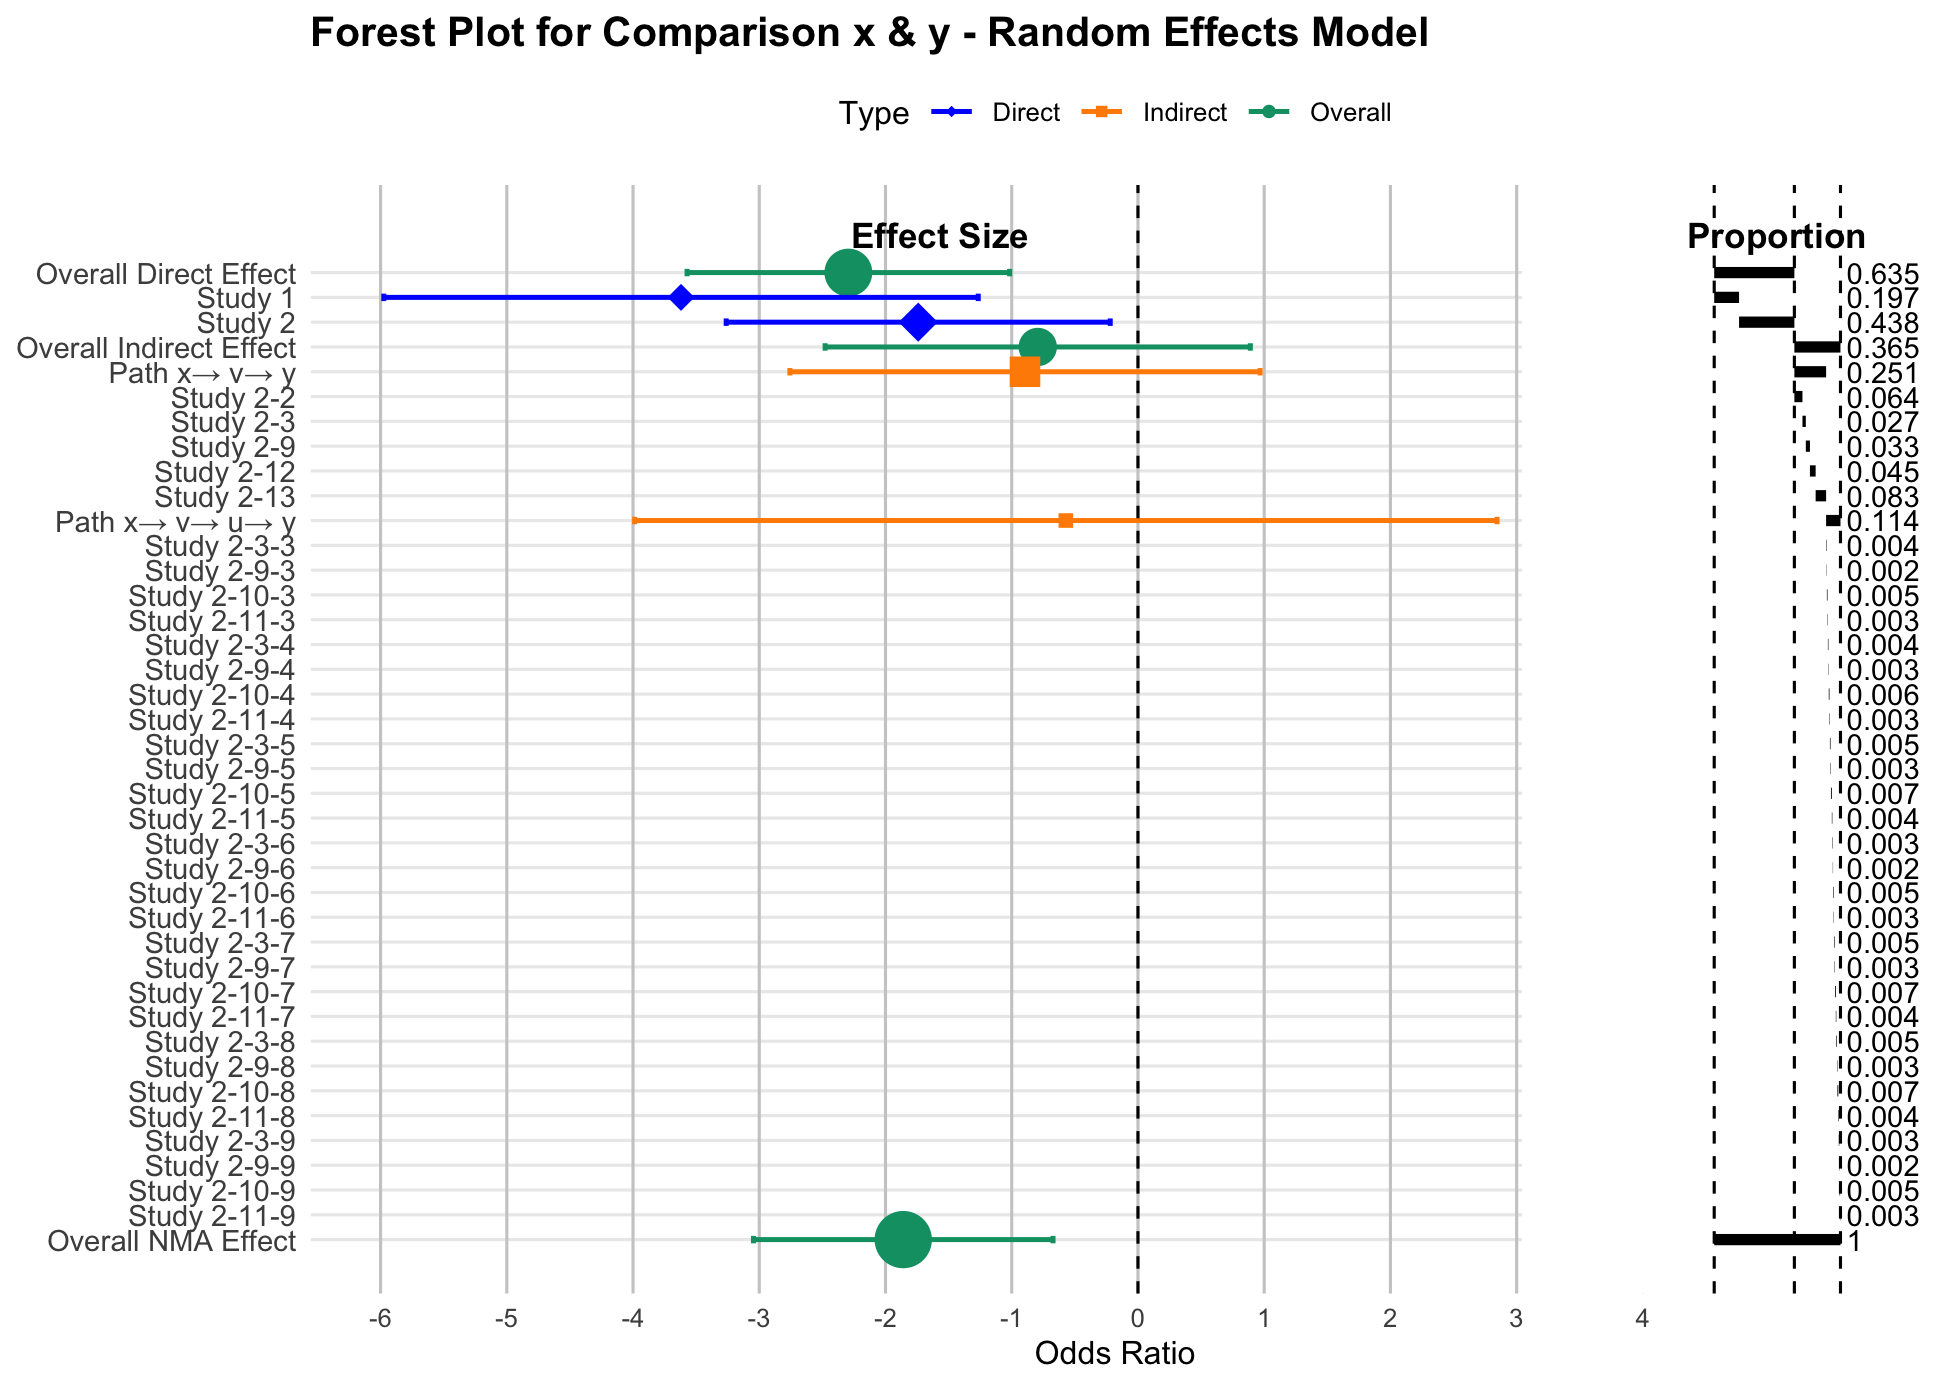
\includegraphics[width=\textwidth]{Rplot1.png}
  \caption{Expanded forest plot for comparison x vs. y, displaying direct, indirect, and overall effects with study-level decomposition of direct and indirect evidence contributions.}
  \label{fig:forestplot1}
\end{figure}

\begin{verbatim}

$output
                     Label EffectSize LowerCI UpperCI     SE weight proportion
1    Overall Direct Effect     -2.294  -3.572  -1.017  0.652  2.353      0.635
2                  Study 1      -3.62  -5.974  -1.265  1.201  0.693      0.197
3                  Study 2     -1.741  -3.262  -0.22   0.776  1.66       0.438
4  Overall Indirect Effect     -0.794  -2.478   0.89   0.859  1.354      0.365
5             Path x→ v→ y     -0.895  -2.757   0.967   0.95  1.108      0.251
6                Study 2-2                                               0.064
7                Study 2-3                                               0.027
8                Study 2-9                                               0.033
9               Study 2-12                                               0.045
10              Study 2-13                                               0.083
11         Path x→ v→ u→ y     -0.571  -3.987   2.845  1.743  0.329      0.114
12             Study 2-3-3                                               0.004
13             Study 2-9-3                                               0.002
14            Study 2-10-3                                               0.005
15            Study 2-11-3                                               0.003
16             Study 2-3-4                                               0.004
17             Study 2-9-4                                               0.003
18            Study 2-10-4                                               0.006
19            Study 2-11-4                                               0.003
20             Study 2-3-5                                               0.005
21             Study 2-9-5                                               0.003
22            Study 2-10-5                                               0.007
23            Study 2-11-5                                               0.004
24             Study 2-3-6                                               0.003
25             Study 2-9-6                                               0.002
26            Study 2-10-6                                               0.005
27            Study 2-11-6                                               0.003
28             Study 2-3-7                                               0.005
29             Study 2-9-7                                               0.003
30            Study 2-10-7                                               0.007
31            Study 2-11-7                                               0.004
32             Study 2-3-8                                               0.005
33             Study 2-9-8                                               0.003
34            Study 2-10-8                                               0.007
35            Study 2-11-8                                               0.004
36             Study 2-3-9                                               0.003
37             Study 2-9-9                                               0.002
38            Study 2-10-9                                               0.005
39            Study 2-11-9                                               0.003
40      Overall NMA Effect     -1.859  -3.046  -0.673  0.605  2.729      1.000
\end{verbatim}

\begin{figure}[htbp]
  \centering
  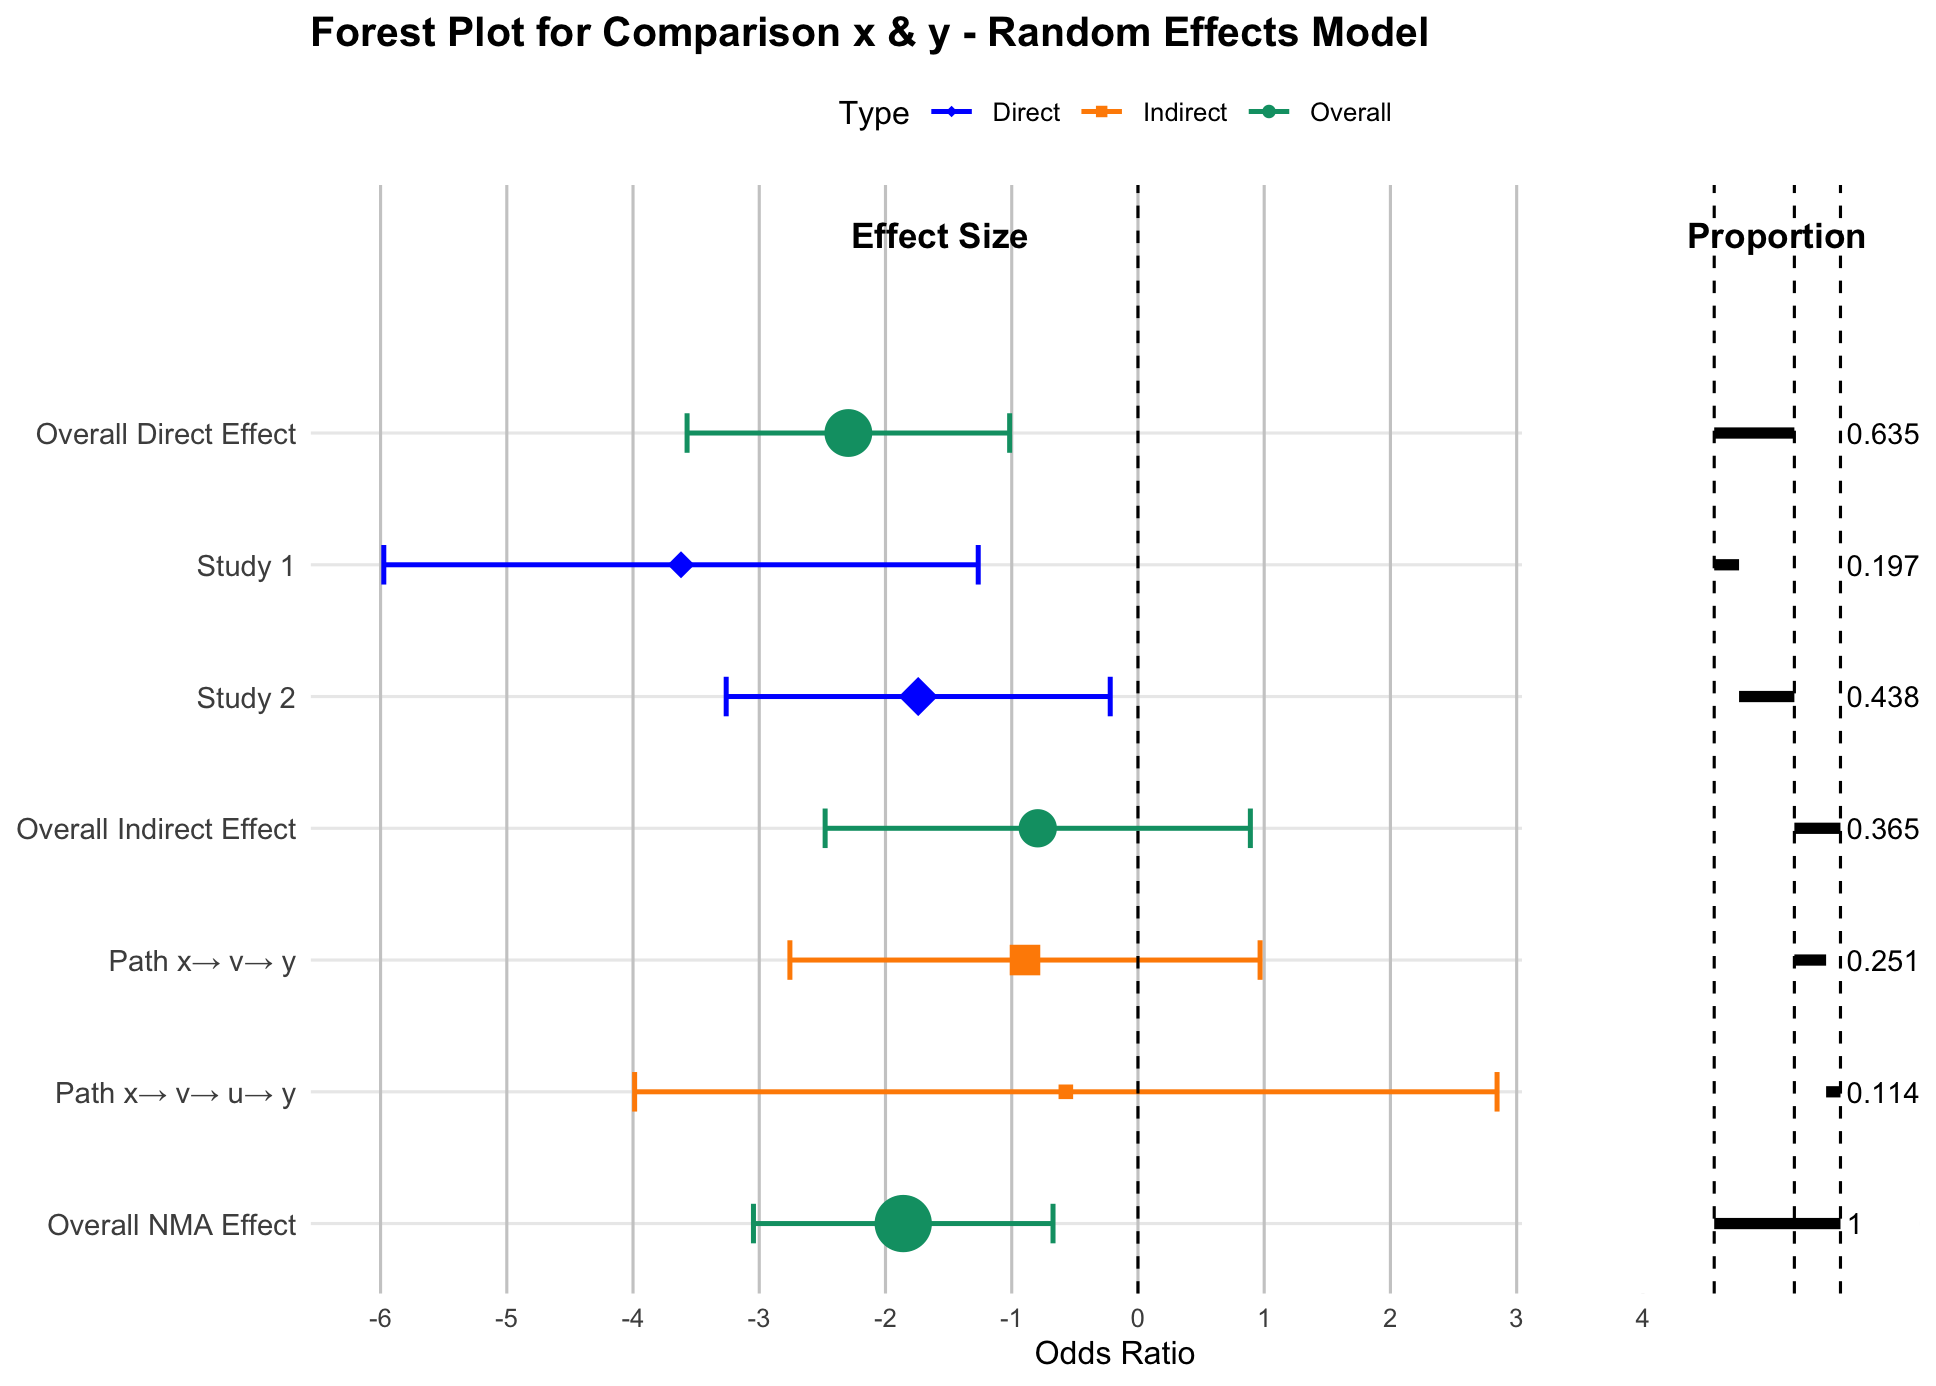
\includegraphics[height=9.88cm]{Rplot2.png}
  \caption{Summary forest plot for comparison x vs. y, displaying direct, indirect, and overall effects without study-combination decomposition. This summary plot corresponds to setting \texttt{study\_path} = \texttt{FALSE} and is particularly useful for large networks where displaying study-combination–level contributions may result in overly dense visualizations.
}
  \label{fig:forestplot2}
\end{figure}

\begin{verbatim}
$output
                    Label EffectSize LowerCI UpperCI     SE weight proportion
1   Overall Direct Effect     -2.294  -3.572  -1.017  0.652  2.353      0.635
2                 Study 1     -3.620  -5.974  -1.265  1.201  0.693      0.197
3                 Study 2     -1.741  -3.262  -0.220  0.776  1.660      0.438
4 Overall Indirect Effect     -0.794  -2.478   0.89   0.859  1.354      0.365
5            Path x→ v→ y     -0.895  -2.757   0.967  0.950  1.108      0.251
6         Path x→ v→ u→ y     -0.571  -3.987   2.845  1.743  0.329      0.114
7      Overall NMA Effect     -1.859  -3.046  -0.673  0.605  2.729      1.000

\end{verbatim}

\paragraph{Note}
For binary outcomes, the summary measure is specified as the odds ratio (\texttt{sm = "OR"} in \CRANpkg{netmeta}). However, estimation is performed on the log-odds ratio scale. Accordingly, effect estimates and confidence intervals displayed in the output tables and forest plots are presented on the log scale.

\subsection{Continuous Data Example Plot and Output}

\begin{figure}[htbp]
  \centering
  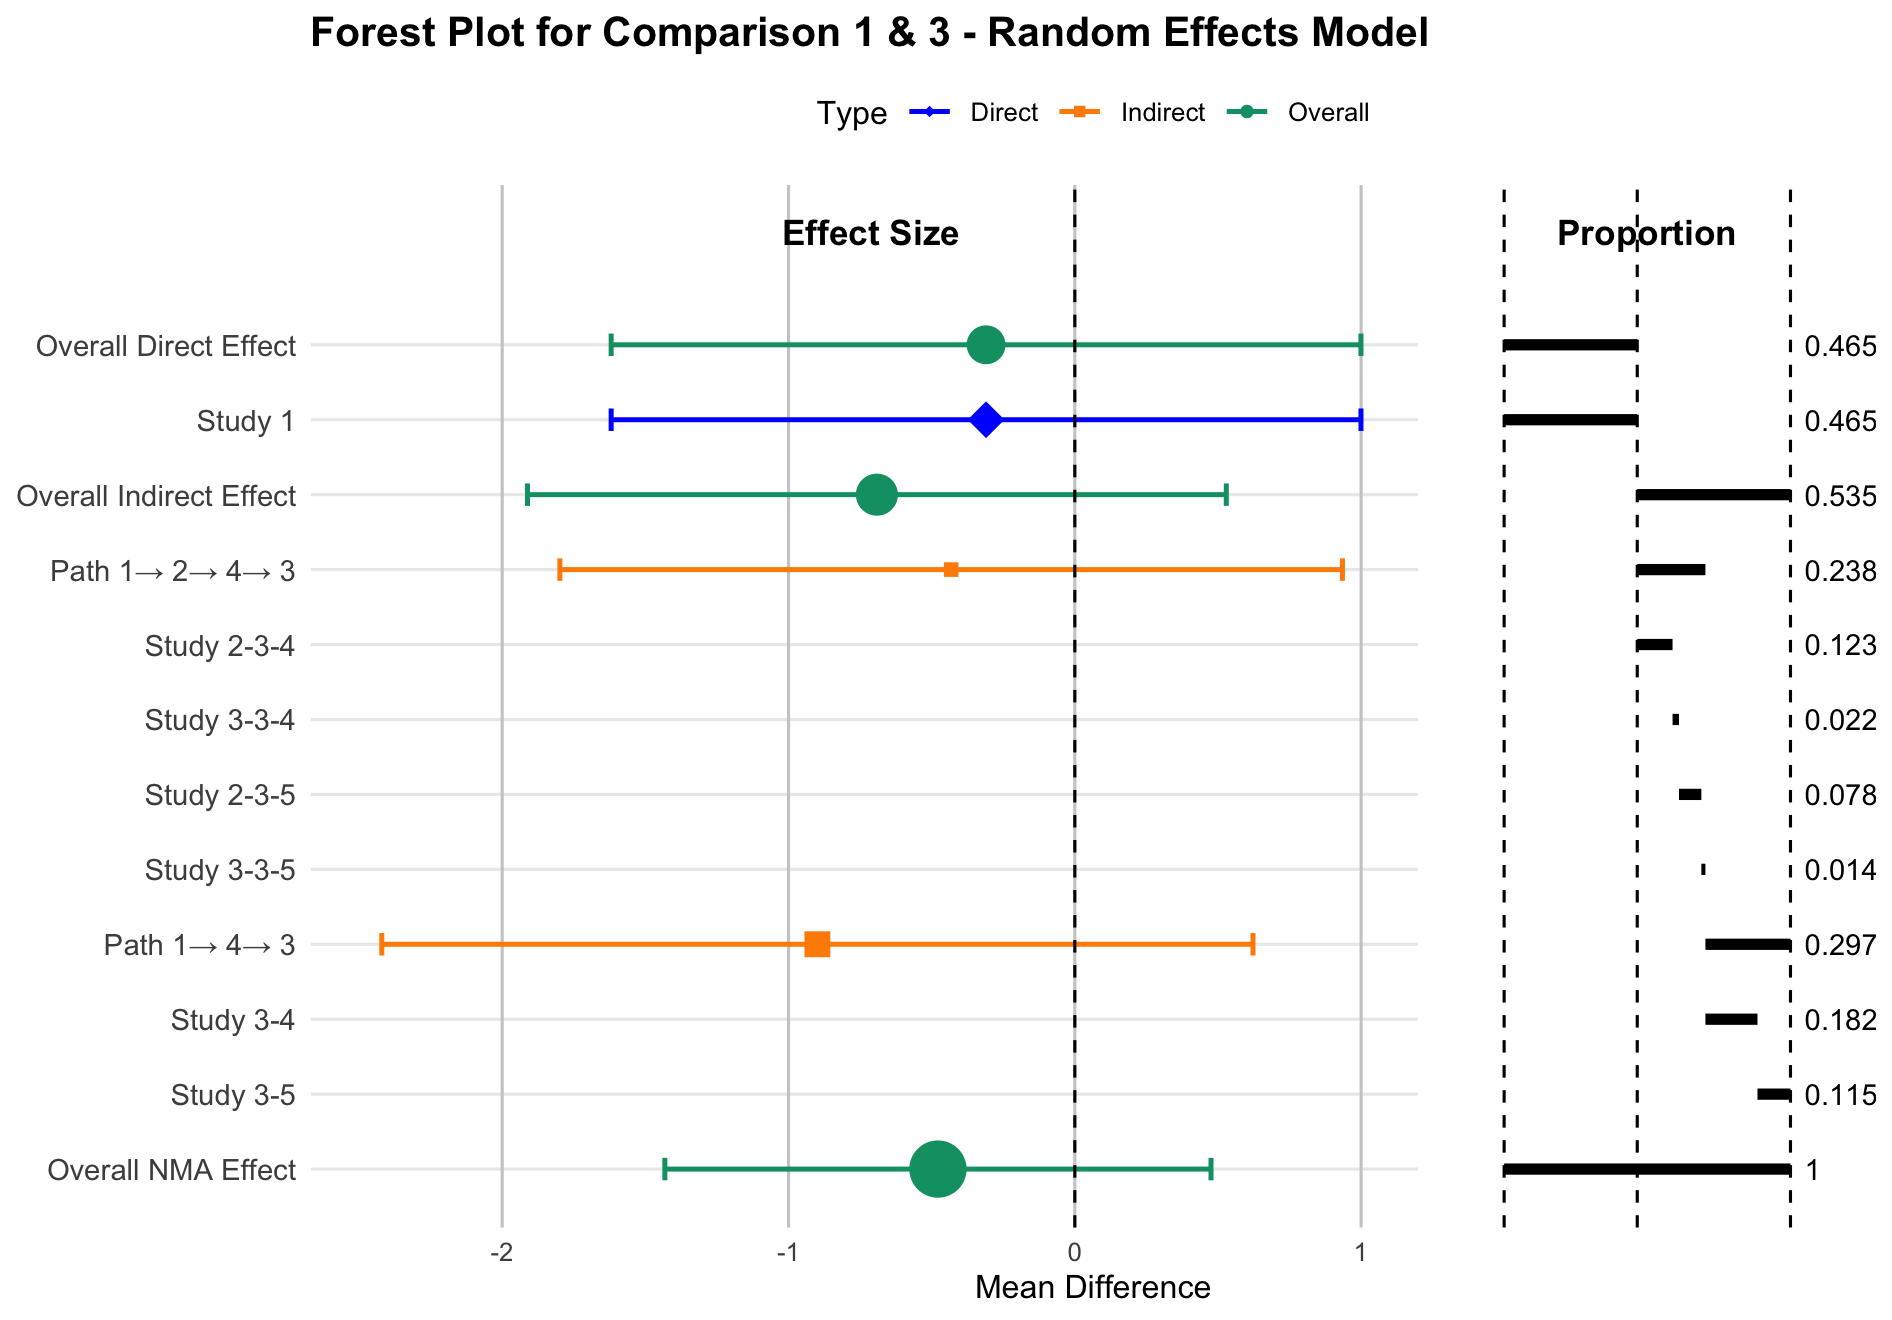
\includegraphics[width=\textwidth]{Rplot3.png}
  \caption{Expanded forest plot for comparison 1 vs. 3, displaying direct, indirect, and overall effects with study-level decomposition of direct and indirect evidence contributions.}
  \label{fig:forestplot3}
\end{figure}

\begin{verbatim}
$output
                     Label EffectSize LowerCI UpperCI     SE weight proportion
1    Overall Direct Effect      -0.31  -1.619   0.999  0.668  2.241      0.465
2                  Study 1      -0.31  -1.619   0.999  0.668   2.24      0.465
3  Overall Indirect Effect     -0.691  -1.912   0.529  0.623  2.579      0.535
4          Path 1→ 2→ 4→ 3     -0.432  -1.799   0.935  0.697  2.057      0.238
5              Study 2-3-4                                               0.123
6              Study 3-3-4                                               0.022
7              Study 2-3-5                                               0.078
8              Study 3-3-5                                               0.014
9             Path 1→ 4→ 3     -0.899  -2.421   0.622  0.776   1.66      0.297
10               Study 3-4                                               0.182
11               Study 3-5                                               0.115
12      Overall NMA Effect     -0.478  -1.432   0.476  0.487  4.223      1.000
\end{verbatim}

\begin{figure}[htbp]
  \centering
  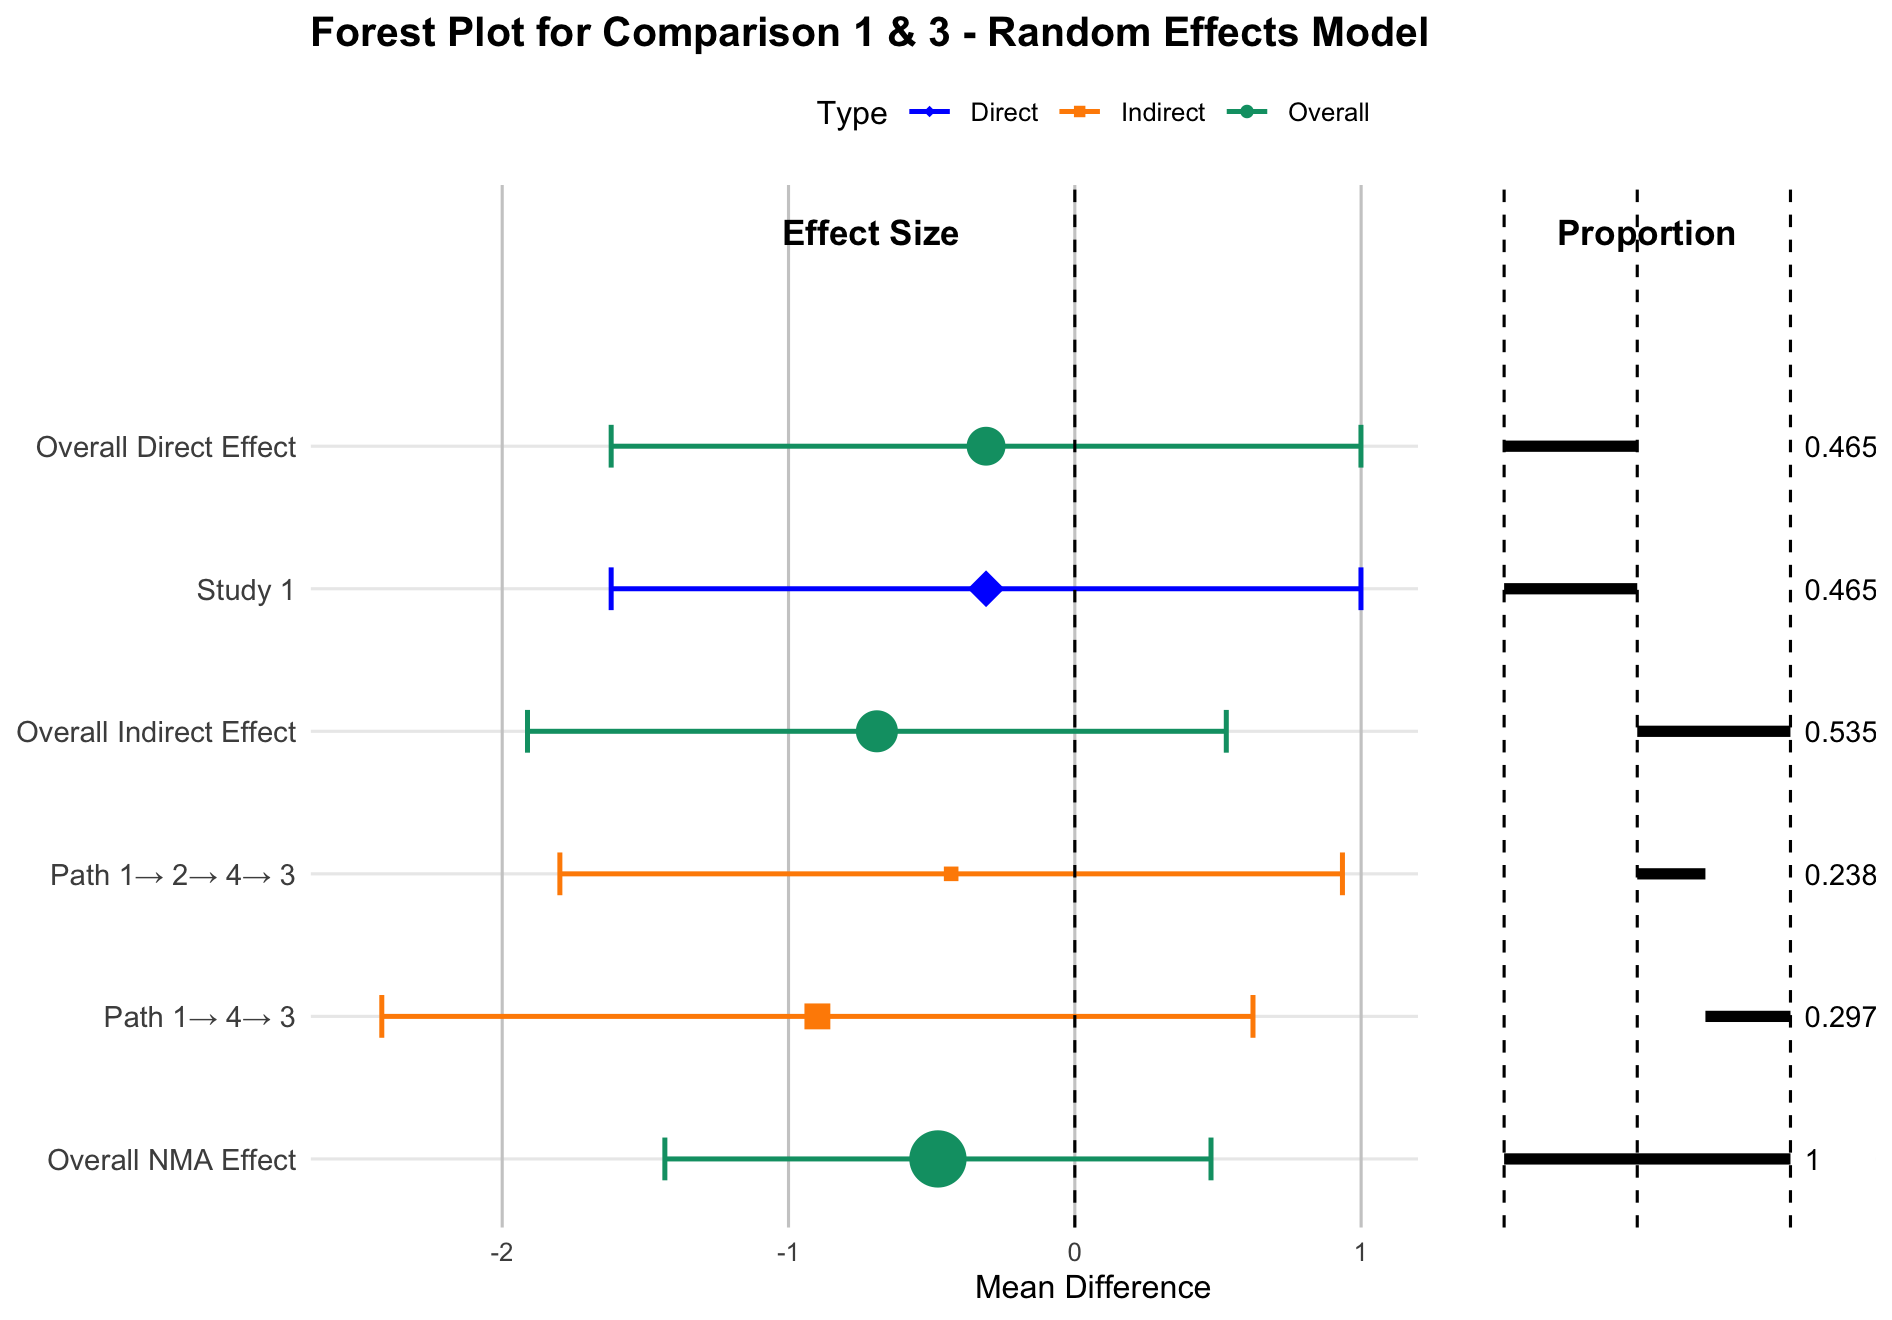
\includegraphics[width=\textwidth]{Rplot4.png}
  \caption{Summary forest plot for comparison 1 vs. 3, displaying direct, indirect, and overall effects without study-combination decomposition. This summary plot corresponds to setting \texttt{study\_path} = \texttt{FALSE} and is particularly useful for large networks where displaying study-combination–level contributions may result in overly dense visualizations.
}
  \label{fig:forestplot4}
\end{figure}

\begin{verbatim}
$output
                    Label EffectSize LowerCI UpperCI     SE weight proportion
1   Overall Direct Effect     -0.310  -1.619   0.999  0.668  2.241      0.465
2                 Study 1     -0.310  -1.619   0.999  0.668  2.240      0.465
3 Overall Indirect Effect     -0.691  -1.912   0.529  0.623  2.579      0.535
4         Path 1→ 2→ 4→ 3     -0.432  -1.799   0.935  0.697  2.057      0.238
5            Path 1→ 4→ 3     -0.899  -2.421   0.622  0.776  1.660      0.297
6      Overall NMA Effect     -0.478  -1.432   0.476  0.487  4.223      1.000
\end{verbatim}

\paragraph{Computational details}

All analyses and example figures reported in this article were generated using
\textsf{R} version~4.4.1. The following main packages were used: \CRANpkg{netmeta}
(version~3.2.0), \CRANpkg{igraph} (version~2.1.4), and \CRANpkg{NMAforest}
(version~0.1.3).

\subsection{Visualizing Decomposition of Evidence}

The \CRANpkg{NMAforest} package provides two styles of forest plots to visualize the composition of treatment effect estimates in a network meta-analysis: an \textbf{expanded version} with full study-level breakdown and a \textbf{summary version} with aggregate-level detail. Both plots help clarify how direct and indirect evidence combine to form the final NMA effect, and how much each evidence component contributes to the result.

The first plot (Figure~\ref{fig:forestplot1}) illustrates a detailed breakdown for the comparison between treatments \texttt{x} and \texttt{y}. It displays:
\begin{itemize}
  \item \textbf{Overall direct effect estimate} with 95\% confidence interval (CI);
  \item \textbf{Study-level direct effect estimates} with 95\% CIs that contribute to the overall direct effect;
  \item \textbf{Overall indirect effect estimate} with 95\% CI;
  \item \textbf{Path-specific indirect effect estimates} with 95\% CIs (e.g., \texttt{x}~$\rightarrow$~\texttt{v}~$\rightarrow$~\texttt{y}, \texttt{x}~$\rightarrow$~\texttt{v}~$\rightarrow$~\texttt{u}~$\rightarrow$~\texttt{y});
  \item \textbf{Study-combination contribution rows} under each path (proportion-only; they share the path’s effect estimate, so SE/CI are omitted);
  \item \textbf{Right-panel proportion bars} indicating the relative contribution of each study, path, or overall component to the effect estimate in the same row.
\end{itemize}

This expanded visualization is especially useful for understanding how indirect comparisons are constructed and which studies dominate specific routes of evidence. Within each indirect path, all study combinations inherit the same path-level effect estimate and uncertainty; therefore, individual effect sizes and confidence intervals are not displayed at the study-combination level.

The second plot (Figure~\ref{fig:forestplot2}) is designed for contexts where clarity and brevity are prioritized. It retains the essential decomposition structure—distinguishing between direct, indirect, and overall NMA effect estimates—while omitting study-level details.
It includes:
\begin{itemize}
  \item \textbf{Overall direct effect estimate} with 95\% CI;
  \item \textbf{Study-level direct effect estimates} with 95\% CIs contributing to the overall direct effect;
  \item \textbf{Overall indirect effect estimate} with 95\% CI, with each indirect path displayed as a single row, without further decomposition into study-combination rows;
  \item \textbf{Overall NMA effect estimate} with 95\% CI;
  \item \textbf{Right-panel proportion bars} aligned with each overall, path-, or study-level estimate, without displaying study-combination contributions.
\end{itemize}

This summary plot is more compact and is well-suited for presentations where space is limited but key decomposition information still needs to be shown, especially in cases where study-level decomposition would be too dense or overwhelming to display in full. In such cases, users are encouraged to set \texttt{study\_path} = \texttt{FALSE}, which suppresses study-level path detail and focuses visualization on aggregated indirect paths, improving clarity without sacrificing key decomposition information.

Both visualizations use color-coded point estimates (blue for study-level direct effect, orange for indirect path effect, and green for overall effect) and horizontal proportion bars. This dual-panel format enables clear interpretation of both statistical magnitude and structural evidence contributions.

\section{Discussion}

The \CRANpkg{NMAforest} package provides a structured and transparent framework for decomposing evidence contributions in network meta-analysis. By combining frequentist estimation outputs from \CRANpkg{netmeta} with graph-based decomposition of indirect evidence flows, it fills a critical gap left by existing tools, which often summarize effect estimates without revealing their sources. This detailed attribution supports users in assessing the robustness and interpretability of treatment comparisons, especially in networks where indirect evidence constitutes a substantial proportion of the overall information.

While the package offers an additional perspective beyond conventional forest plots, several limitations merit consideration. First, the current implementation relies on a constant correlation coefficient to approximate covariance between indirect path segments, which may oversimplify dependencies, particularly in the presence of multi-arm studies or sparse evidence structures. Second, although the visualization of study combinations within indirect paths provides a high level of granularity, it can result in complex or crowded displays when networks are large. To address this, the package includes an option that allows users to suppress the study-combination detail and display only the aggregated contributions of each indirect path, thereby balancing interpretability and comprehensiveness according to the needs of the analysis.

Future enhancements could further improve flexibility by exploring alternative methods for covariance estimation, incorporating Bayesian models of network meta-analysis, and developing interactive visualization features that allow users to filter, collapse, or highlight specific evidence contributions dynamically.

\section{Conclusion}

\CRANpkg{NMAforest} package provides a clear and practical approach for linking treatment effect estimates with their contributing studies and indirect evidence paths in network meta-analysis. By offering contribution-aware visualizations alongside standard effect summaries, the package supports more transparent reporting and helps users interpret the origins of their results with greater confidence. We believe this approach will facilitate clearer communication of evidence synthesis findings across research and applied decision-making contexts.

\bibliography{NMAforest_RJournal}

\address{Yanqi Zhang\\
  Department of Statistics\\
  Iowa State University\\
  2438 Osborn Dr Ames, IA 50011-1090\\
  United States\\}
\email{zyq1998@iastate.edu}

\address{Chong Wang\\
  Professor, Department of Veterinary Diagnostic and Production Animal Medicine, Department of Statistics\\  Iowa State University\\
  2239 Lloyd Vet Med Ctr Ames, IA 50011-3619\\
  United States\\}
\email{chwang@iastate.edu}

\address{Annette O’Connor\\
 Professor,  Department of Large Animal Clinical Sciences\\
  Michigan State University\\
  Veterinary Medicine Center
736 Wilson Road, Room D-202
East Lansing, MI 48824\\
  United States\\}
\email{oconn445@msu.edu}
